\documentclass[a4paper,10pt]{scrbook}
\usepackage{etex}
\usepackage[T1]{fontenc}
\usepackage{geometry}
\usepackage[utf8x]{inputenc}
\usepackage[ngerman]{babel}
\usepackage{graphics}
\usepackage{graphicx}
\usepackage{amssymb}
\usepackage{amsmath}
\usepackage{listings}
\usepackage{booktabs}
\usepackage{pdfpages}
\usepackage{pgfplots}
\usepackage{float}
\usepackage{latexsym}
\usepackage{longtable}
\usepackage{latexsym}
\usepackage{paralist}
\usepackage{enumitem}
\usepackage{pstricks}
\usepackage{stmaryrd}
\usepackage{MnSymbol}
\usepackage{array}
\usepackage{linearb}
\usepackage{titlesec}
\usepackage{listings}
\usepackage{xcolor}
\usepackage{xspace} 
\usepackage{hyperref} 
\usepackage{enumitem}

%Für Arrow listen
\newlist{arrowlist}{itemize}{1}
\setlist[arrowlist]{label=$\rightarrow$}


%Mehr Raum zwischen subsections
\titlespacing{\section}{0pt}{*4}{*2.5}
\titlespacing{\subsection}{0pt}{*3.5}{*1.5}

% kleine Anpassungen, damit die Seitenbreite überall außer Titel gleich ist.
\setcounter{secnumdepth}{2}
\setlength{\textwidth}{160mm}
\setlength{\textheight}{220mm}
\setlength{\headheight}{3mm}
\evensidemargin1mm
\oddsidemargin1mm

%Subsubsections werden hiermit nicht in das Inhaltsverzeichnis übernommen
\setcounter{tocdepth}{2}


%Dokumentenanfang mit diversen input von mehreren Einzeldokumenten.
\begin{document}
	\begin{titlepage}
\center
\Large Software Engineering\large \\[2em]
Lernskript \\[2em]
Dozent:\\Prof. Dr. Stefan Kramer\\[2em]
\LaTeX{} von:\\Sven Bamberger\\[2em]
Zuletzt Aktualisiert:\\\today\\

\includegraphics[scale=.2]{front/pics/Logo.jpg}\\\quad\\
\end{titlepage}
 
	
	\frontmatter 
		Dieses Skript wurde erstellt, um sich besser auf die Klausur vorzubereiten.\\
\qquad\\
\qquad\\
\textcolor{red}{\Large{Dieses Dokument garantiert weder Richtigkeit noch Vollständigkeit, da es aus Mitschriften und Vorlesungsfolien gefertigt wurde und dabei immer Fehler entstehen können. Falls ein Fehler enthalten ist, bitte melden oder selbst korrigieren und neu hoch laden.}}


		 
\tableofcontents 
 
	 
	\mainmatter 
	    \chapter{Zusammenfassung - Lernziele}
\begin{itemize}
    \item \textbf{Software Engineering ist eine Ingenieursdisziplin, die sich mit allen Aspekten der Softwareproduktion beschäftigt}
    \item High-level activities specifications, Entwicklung, Validierung und Evolution sind Teil aller Softwareprozesse.
    \item Prozesse:
    \begin{itemize}
        \item Wasserfallmodell
        \item V-Modell
        \item Boehm's spiral model
        \item RUP (modernes generisches Prozessmodell)
        \item agile Methoden (Scrum, XP, \dots),\dots
    \end{itemize}
    \item Es gibt \textbf{viele verschiedene Systemformen}, ihre Entwicklung erfordert eigene Software Engineering-Tools und Techniken 
    \item \textbf{Requirements engineering} ist der Prozess der Entwicklung einer Software-Spezifikation 
    \begin{itemize}
        \item Kernpunkte: User- und System Requirements, Funktionale und nicht funktionale Anforderungen, Qualitätseigenschaften der Anforderungen
    \end{itemize}
    \item Design: \textbf{high-level design} (architectural design) und \textbf{low-level design}
    \begin{itemize}
        \item Pattersn als Weg, bekannte, erfolgreiche Designstrategien zu übertragen
    \end{itemize}
    \item \textbf{Verfication und Validation:} Inspecktion (\textit{code reviews}) und Testen (viele Verschiedene Formen des Testings:
    \begin{itemize}
        \item defect testing
        \item validation testing
        \item unit testing
        \item component testing
        \item system testing
        \item regression testing
        \item \dots
    \end{itemize}
    \item Project Management
    \begin{itemize}
        \item Einhaltung des Zeitplans und des Budgets
        \item \textbf{Risikomanagement} gilt als einer der wichtigsten Punkte, Hauptwerkzeug: Notfallplan
        \item Personalmangement: Bedürfnishierachie, Persönlichkeitstypen
    \end{itemize}
    \item Project planning
    \begin{itemize}
        \item Milestones, deliverables, Gantt (or activity bar) chart
        \item \textbf{Kostenabschätzung COCOMO2}
    \end{itemize}
    \item Quality mangement 
    \begin{itemize}
        \item \textbf{Prüfplan, ISO 9001-Standart, software metrics }
    \end{itemize}
    \item \textbf{CMMI-Modell für Prozessoptimierung}
\end{itemize}

		\chapter{Introduction to Software Engineering}
\section{Was versteht man unter Software-Engineering?}
\textbf{Software Engineering} ist eine Ingenierusdisziplin, die sich mit allen Aspekten der Softwareherstellung beschäftigt.
\section{Technische Disziplin:}
\begin{itemize}
    \item Techniker wenden Methoden, Werkzeuge und Theorien an um Dinge zum Laufen zu bringen
    \item Techniker erkennen an, dass sie mit oganisatorischen und finanziellen Beschränkungen arbeiten müssen
\end{itemize}
\section{Alle Aspekte der Softwareherstellung:}
\begin{itemize}
    \item SE beschäftigt sich nicht nur mit technischen Prozessen der Softwareentwicklung
    \item auch Projektverwaltung und Entwicklung von Werkzeugen, Methoden und Theorien, welche die Sofwareherstellung unterstützen
\end{itemize}
\section{Softwareprozess (grundlegende Aktivitäten von SE):}
\begin{itemize}
    \item Softwarespezifikation
    \begin{itemize}
        \item Kunden und Entwickler definieren die zu produzierende Software und die Rahmenbedingung fr ihren Einsatz
    \end{itemize}
    \item Softwareentwicklung
    \begin{itemize}
        \item Software wird entworfen und programmiert
    \end{itemize}
    \item Softwarevalidierung (Softwarebeurteilung):
    \begin{itemize}
        \item Software wird überprüft um sicherzustellen, dass sie den Kundenanforderungen entspricht
    \end{itemize}
    \item Softwareevolution
    \begin{itemize}
        \item Software wird weiterentwickelt, damit sie die sich ändernden Bedürfnisse der Kunden und des Marktes wiederspiegelt
    \end{itemize}
\end{itemize}

\section{Software-Produkte}
\begin{itemize}
    \item \textbf{Generisch:} Stand-alone-Systeme, dei vermakted und an jeden Interessenten verkauft werden
    \begin{itemize}
        \item Beispielsweise: Software für den PC, Datenbanken, Textverarbeitungsprogramme
    \end{itemize}
    \item \textbf{Produktspezifikation:}
    \begin{itemize}
        \item Anforderungen werden vom Entwickler definiert, Entscheidungen über Änderungen werden vom Entwickler getroffen.
    \end{itemize}
    \item \textbf{Kundenindividuell:} Software die im Auftrag eines bestimmten Kunden hergestellt werden
    \begin{itemize}
        \item Biespielsweise: Steuerungssysteme für elektronische Geräte, System zur Unterstützung eines bestimmten Geschäftprozesses
    \end{itemize}
    \item \textbf{Produktspezifkation:}
    \begin{itemize}
        \item Anforderungen werden vom Kunden definiert, Entscheidungen über notwendige Änderungen der Software werden vom Kunden getroffen
    \end{itemize}
\end{itemize}

\section{Unterschiede dieser Softwaretypen:}
\begin{itemize}
    \item Allgemeine Produkte:
    \begin{itemize}
        \item Unternehmen, das Software entwickelt, bestimmt die Spezifikationen der Software
    \end{itemize}
    \item Angepasste Produkte:
    \begin{itemize}
        \item Spezifikation wird von dem Kunden entwickelt und kontrolliert, dass das System kauft
    \end{itemize}
\end{itemize}

\section{Viele unterschiedliche Anwendungsarten:}
\begin{itemize}
    \item Eigenständige (stand-alone) Anwendungen:
    \begin{itemize}
        \item Softwware läuft lokal
        \item Beinhaltet alle notwendigen Funktionen um ohne Netzwerkverbindung zu laufen
        \item z.B. Fotoanwendungen ohne Netzwerkzugriff
    \end{itemize}
    \item Interaktive transaktionsbasierte Anwendungen:
    \begin{itemize}
        \item laufen auf externen PC's und werden vom User aufgerufen
        \item Webapplikationen über Cloud-Zugriff
    \end{itemize}
    \item Eingebettete Steuerungssysteme:
    \begin{itemize}
        \item es gibt daon mehr als von allen andern Anwendungsarten
        \item Software für ABS im Auto
        \item Kontrollieren die Hardware
    \end{itemize}
    \item Stapelverarbeitende Systeme (Batch-Verarbeitungssysteme)
    \begin{itemize}
        \item Systeme die große Datenmengen verarbeiten (z.B. Business-Systeme)
        \item Abrechnung von regelmäßigen Zahlungen (Telefonrechnung)
    \end{itemize}
    \item Unterhaltungssysteme
    \begin{itemize}
        \item zum persönlichen Gebrauch
        \item z.B. Spiele
    \end{itemize}
    \item Systeme für die Modellierung und Simulation
    \begin{itemize}
        \item Systeme, die von Wissenschaftlern und Ingenieuren entwickelt wurden
        \item z.B. physikalische Prozesse simulieren
    \end{itemize}
    \item Datenerfassungssysteme
    \begin{itemize}
        \item System, welches Daten unter extremen Bedingungen mit Hilfe von Sensoren erfassen und weiterleiten
    \end{itemize}
    \item Systeme von Systemen
    \begin{itemize}
        \item Zusammensetzung von vielen Softwaresystemen
    \end{itemize}
\end{itemize}

\section{Software Engineering FAQ}

\begin{enumerate}
    \item Software Definition
    \begin{itemize}
        \item Computerprogramme und dazugehörige Dokumentationen können für bestimmte 
    \end{itemize}
    \item Attribute guter Software 
    \begin{itemize}
        \item Liefert geforderte Funktionalität und Leistung, ist wartbar, zuverlässig, effizient und benutzbar
    \end{itemize}
    \item Software Engineering Definition 
    \begin{itemize}
        \item Ingenieursdiziplin, die sich mit allen Aspekten der Softwareproduktion befasst. 
    \end{itemize}
    \item Software Enigneering: Grundsätzliche Tätigkeiten
    \begin{itemize}
        \item Software-Spezifikation, Entwicklung, Validierung, Evolution
    \end{itemize}
    \item Unterschied Software Engineering $\leftrightarrow$ Systementwicklung
    \begin{itemize}
        \item Informatik: Theorie und Grundlagen
        \item Softwareentwicklung: Praktisches Umsetzung der Entwicklung und Auslieferung nützlicher Software 
    \end{itemize}
    \item Unterschied Software Engineering $\leftrightarrow$ Systementwicklung 
    \begin{itemize}
        \item Systementwicklung beinhaltet alle Aspekte computerbasierter Entwicklung, Hardware-, Software-, Prozessentwicklung
    \end{itemize}
    \item Zentrale Herausforderungen des Software Engineerings
    \begin{itemize}
        \item zunehmende Vielfalt, Forderung verkürzter Lieferzeiten, Entwicklung vertrauenswürdiger Software
    \end{itemize}
    \item Kosten des Software Engineerings 
    \begin{itemize}
        \item 60\% Entwicklung, 40\% Testing
    \end{itemize}
    \item Beste Techniken und Methoden
    \begin{itemize}
        \item passende Techniken für unterschiedliche Systemarten 
    \end{itemize}
    \item Einfluss des WWW 
\end{enumerate}
\section{Wesentliche Merkmale guter Software:}
\begin{itemize}
    \item Wartbarkeit
    \begin{itemize}
        \item kritisches Merkmal 
        \item Software sollte so geschrieben werden, dass sie \textbf{weiterentwickelt werden kann}, um sich verändernden Kundenbedüfnissen Rechnung zu tragen
        \item Softwareanpassungen sind eine unvermeidliche Anforderung einer sich verändernden Geschäftsumgebung 
    \end{itemize}
    \item Verlässlichkeit (dependability) und Informationssicherheit (security):
    \begin{itemize}
        \item Verlässliche Software sollte keinen körperlichen oder wirtschaftlichen Schaden verursachen, falls das System ausfällt
        \item Böswillige Benutzer sollten nicht in der Lage sein, auf das System zuzugreifen oder es zu beschädigen
    \end{itemize}
    \item Effizienz (efficiency):
    \begin{itemize}
        \item Software sollte nicht verschwenderisch mit Systemressourcen wie Speicher und Prozessortkapazität umgehen
        \item Effizien umfasst somit Reaktionszeit, Verarbeitungszeit, Speichernutzung usw. 
    \end{itemize}
    \item Akzeptanz (acceptability)
    \begin{itemize}
        \item Software muss von den Benutzern akzeptiert werden, für die sie entwickelt wurde. Das bedeutet, dass sie verständlich, nützlich und kompatibel mit anderen Systemen sein müssen, die diese Benutzer verwenden.
    \end{itemize}
\end{itemize}

\section{Grundsätze des Software Engineering:}
\begin{itemize}
\item Einsatz eines kontrolliertern, vereinbarten Entwicklungsprozesses
\item Zuverlässigkeit und Leistungsfähigkeit wichtig
\item Verständnis und Kontrolle der Software-Spezifikation und der Anforderungenen sind wichtig
\item Wiederverwendung bereits vorhandener Software sollte der Vorzug vor der Entwicklung neuer Soft-ware vorgezogen werden.
\end{itemize}

\section{Key points}
\begin{enumerate}
    \item Softwareentwicklung ist eine Ingenieursdisziplin, die sich mit allen Aspekten der Softwareproduktion beschäftigt. 
    \item Wesentliche Attribute eines Software-Produktes sind Wartbarkeit, Zuverlässigkeit und Sicherheit, Effizienz und Abnahmefähigkeit.
    \item high-level-Aktiviäten der Spezifikation, Entwicklung, Validierung und Evolution sind Teil aller Softwareprozesse.
    \item Grundlegende Ideen der Softwareentwicklung sind universell andwendbar auf alle Formen von Systementwicklung.
    \item Jede Art von System erfordert passende Entwicklungs-Tools.
    \item Die grundlegende Ideen der Softwareentwicklung sind anwendbar für alle Formen von Sostwaresystemen. 
\end{enumerate}

		\chapter{Softwareprozesse}
Softwareprozess ist eine Menge von zusammengehörigen Aktivitäten, die zur Produktion eines Softwareprodukts führen.
\section{Vier Aktivitäten die grundlegend für SE sind:}
\begin{itemize}
    \item Softwarespezifikation:
    \begin{itemize}
        \item Beschreibung was das System macht
    \end{itemize}
    \item Softwareentwurf und -implementierung
    \begin{itemize}
        \item Definieren des Systemaufbaus
        \item Implementierung des Systems
    \end{itemize}
    \item Softwarevalidierung
    \begin{itemize}
        \item Sind Kundenwünsche erfüllt
    \end{itemize}
    \item Softwareevolution
    \begin{itemize}
        \item Weiterentwicklung und eingehen auf veränderte Bedürfnisse des Kunden
    \end{itemize}
\end{itemize}

\section{Plangesteurte und agile Prozesse:}
\begin{itemize}
    \item Plangesteurte Prozesse:
    \begin{itemize}
        \item Verfahren bei denen alle Prozessaktivitäten im Voraus geplant werden
        \item Fortschritte werden an dem Plan gemessen
    \end{itemize}
    \item Pro:
    \begin{itemize}
        \item durch frühzeitige Planung werden Probleme und Abhängigkeiten entdeckt\\
         (z.B. Personalbedarf)
    \end{itemize}
    \item Contra:
    \begin{itemize}
        \item viele frühe Entscheidungen müssen korrigiert werden \\
        (z.B. wegen Änderungen in der Umgebung)
    \end{itemize}
    \item Agile Prozesse:
    \begin{itemize}
        \item Planen ist inkrementell und es ist einfacher Prozesse zu verändern 
    \end{itemize}
    \item Es muss eine Balance zwischen beiden Prozessen gefunden werden
\end{itemize}

\section{Vorgehensmodelle (Softwareprozessmodelle):}
\begin{itemize}
    \item Wasserfallmodell
    \item Inkrementelle Entwicklung 
    \item Wiederverwendungsorientierte SE
\end{itemize}

\subsection{Wasserfallmodell:}
\begin{figure}[h] 
  \centering
     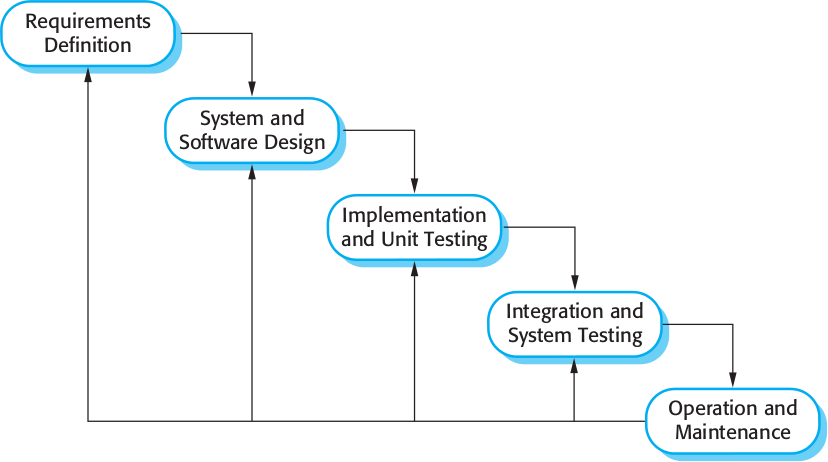
\includegraphics[width=0.75\textwidth]{mainmatter/pics/waterfall.png}
  \caption{Wasserfallmodell: Plangesteuerter Prozess}
\end{figure}
\begin{itemize}
    \item Modell stellt die grundlegende Prozessabläufe (Spezifikation, Entwicklung, Validierung und Evolution) als eigene Phase des Prozesses dar
    \item Phasen
    \begin{enumerate}
        \item Analyse und Definition der Anforderungen dienen als Systemspezifikation
        \item System- und Softwareentwurf:
        \begin{itemize}
            \item Übergeordnete Systemarchitektur wird festgelegt
            \item Erkennen und Beschreiben  der grundlegenden abstrakten Softwaresysteme 
        \end{itemize}
        \item Implementierung und Modultests
        \item Integration und Systemtest
        \begin{itemize}
            \item System wird als Ganzes getestet zur Siherheitsstellung, dass die Softwareanforderungen erfüllt sind. 
        \end{itemize}
        \item Betrieb und Wartung
    \end{enumerate}
    \item Hauptproblem ist die starre Aufteilung des Projekts in verschiedene Phasen
    \item Man kann nicht gut auf neue Anforderungen des Kunden reagieren
    \item gute \glqq{}Wahl\grqq{}, wenn Anforderungen gut durchdacht sind und wenn keine Änderungen zu erwarten sind
    \item geeignet für große Systeme
\end{itemize}

\subsection{Inkrementelle Entwicklung}
\begin{itemize}
    \item Spezifikation, Entwicklung und Validierung sind verschachtelt. Kann sowohl plangesteuertals auch agil sein.
    \item System wird als eine Folge von Versionen (Inkrementen) entwickelt, wobei jede Version neue Funktionalität zu der vorherigen hinzufügt
    \item Spezifikation, Entwicklung und Validierung werden gleichzeitig ausgeführt
\end{itemize}
\begin{figure}[h] 
  \centering
     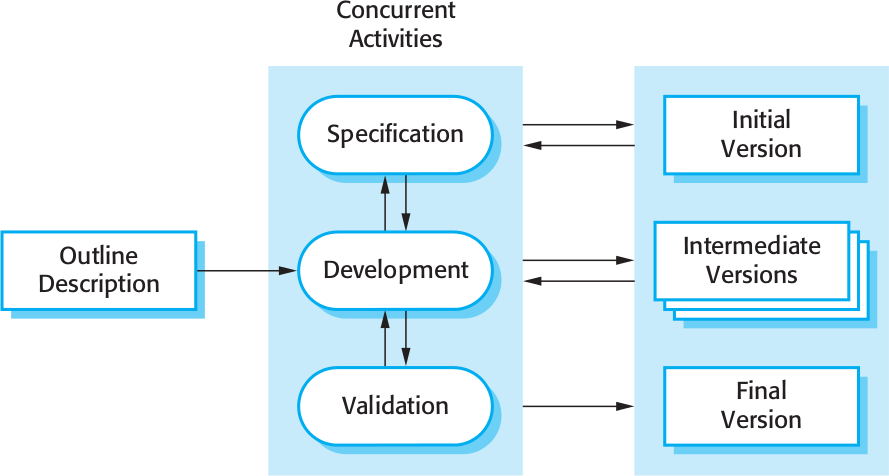
\includegraphics[width=0.75\textwidth]{mainmatter/pics/inkrement_evolution.png}
  \caption{Inkrementelle Entwicklung}
\end{figure}
\textbf{Vorteile inkrementelle Entwicklung (gegenüber Wasserfallmodell):}
\begin{itemize}
    \item Kosten für Kundenanforderungsänderungen werden reduziert
    \item Es ist einfacher Kundenrückmeldungen zu bekommen 
    \item Schnellere Auslieferung an den Kunden von verwendungsfähiger Software 
\end{itemize}

\textbf{Nachteile inkrementelle Entwicklung}
\begin{itemize}
    \item Prozess ist nicht sichtbar
    \begin{itemize}
        \item Fortschritt nicht messbar
    \end{itemize}
    \item Systemstruktur wird tendenziell schwächer, wenn neue Inkremente hinzugefügt werden
\end{itemize}
\subsection{Inkrementelle Lieferung}
\begin{itemize}
    \item Entwicklung und Auslieferung werden in mehrere Schritte aufgeteilt, jeder Schritt liefert einen Teil der geforderten Funktionalitäten
    \item Den Benutzeranforderungen werden Prioritäten zugewiesen, die Anforderungen mit höherer Priorität werden in früheren Schritten bearbeitet 
    \item während der Bearbeitung eines Schrittes werden die betreffenden Anforderungen nicht mehr verändert
\end{itemize}
\begin{figure}[h] 
  \centering
     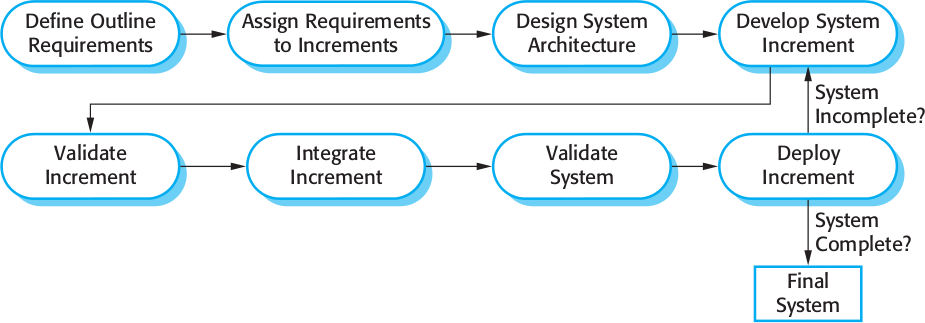
\includegraphics[width=0.75\textwidth]{mainmatter/pics/inkrement_delivery.png}
  \caption{Inkrementelle Lieferung}
\end{figure}
\textbf{Vorteile:}
\begin{itemize}
    \item Schrittweise gelieferte Systemfunktionalität
    \item Frühe Schritte dienen als Vorlage, mit der spätere Schritte bestimmt werden
    \item Geringes Risiko für Fehlschlag der gesamten Software 
    \item die hoch priorisierten Systemdienstleistungen werden oft getestet
\end{itemize}
\textbf{Nachteile:}
\begin{itemize}
    \item Schwer zu verwalten
\item  Systemstruktur wird aufgeweicht
\item  Kompatibilität mit Geschäftsprozessen auf Kundenseite nicht gesichert
\item  Ersetzen eines bestehenden Systems problematisch $\rightarrow$ Schritte enthalten weniger Funktionalität
\end{itemize}

\subsection{Wiederverwendungsorientiertes Software Engineering}
\begin{figure}[h] 
  \centering
     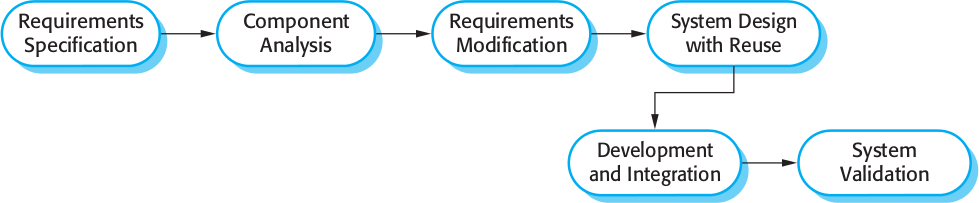
\includegraphics[width=0.75\textwidth]{mainmatter/pics/reused.png}
  \caption{Reuseoriented software engineering}
\end{figure}


\begin{itemize}
    \item beides (Plandriven \& agiler Prozess)
    \item basiert auf Existenz einer beträchtlichen anzahl von wiederverwendbaren Komponenten 
    \item Prozessstufen: 
    \begin{itemize}
        \item Komponenten Analyse
        \item Anforderungsmodifikation
        \item Systementwurf mit Wiederverwendung 
        \item Entwicklung und Integration
    \end{itemize}
    \item meist aus allen Modellen zusammengesetzt
\end{itemize}

\subsection{Typen der Software-Komponenten:}
\begin{itemize}
    \item Stand-Alone-Software (COTS Commercial-off-the-shelf):\\
    wurde für den Einsatz in einer bestimmten Umgebung Entwickelt
    \item Sammlung von Objekten, die als Paket mit einem Komponentenframework wie .NET oder J2EE integriert und entwickelt wurden
    \item Web-Services:\\
    wurden je nach Servicestandard entwickelt und für Remote-Aufrufe verfügbar gemacht
\end{itemize}

\section{Prozessaktivitäten:}
\subsection{Softwarespezifikation}
Prozess zum Verstehen und Definieren der vom System verlangten Funktion sowie der Beschränkungen, denen der Betrieb und die Entwicklung des Systems unterliegen. 
\\
\textbf{Requirements Engineering}
\begin{enumerate}
    \item Anforderungsanalyse besteht aus 
    \item \textbf{Durchführbarkeitsstudie:}
    \begin{itemize}
        \item Ist es aus technischer und finanzierler Sicht möglich das System zu entwickeln?
    \end{itemize}
    \item \textbf{Erhebung und Analyse der Anforderungen:}
    \begin{itemize}
        \item Was erwarten die Kunden von dem System 
    \end{itemize}
    \item \textbf{Spezifikation der Anforderungen:}
    \begin{itemize}
        \item Definieren der Anforderungen im Detail
    \end{itemize}
    \item \textbf{Validierung der Anforderungen:}
    \begin{itemize}
        \item Sind die Anforderungen realistisch, konsistent und vollständig?
    \end{itemize}
\end{enumerate}
\begin{figure}[h] 
  \centering
     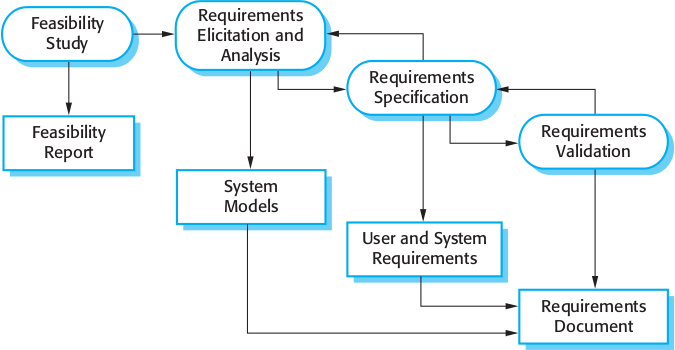
\includegraphics[width=0.75\textwidth]{mainmatter/pics/requ.png}
  \caption{Softwarespezifikationen}
\end{figure}

\subsection{Design und Implementierung}
Umwandlen der Spezifikationen in ein ausführbares System.
\begin{itemize}
\item Software-Design
    \begin{itemize}
        \item  Entwicklung einer Softwarestruktur, die die Spezifikation umsetzt.
    \end{itemize}
\item Implementierung
    \begin{itemize}
        \item Übersetzung der Struktur in ein ausführbares Programm.
    \end{itemize}
\end{itemize}
\begin{figure}[h] 
  \centering
     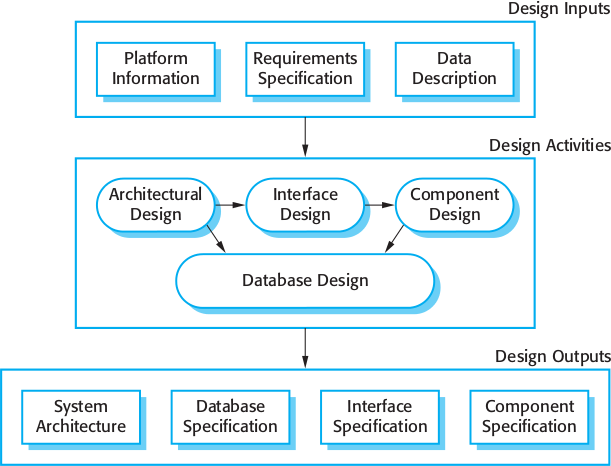
\includegraphics[width=0.75\textwidth]{mainmatter/pics/entw_impl.png}
  \caption{Design und Implementierung}
\end{figure}

\subsection{Designaktivitäten
}
\begin{itemize}
    \item Architekturentwurf:\\
    Gesamtstruktur des Systems $\rightarrow$ Hauptkomponenten (wie Untersysteme und Module), Beziehungen und deren Verteilungen
    \item Schnittstellenentwurf:\\
    Definition der Schnittstellen zwischen Systemkomponenten
    \item Komponentenentwurf:\\
    Jede Komponente und jedes Design wird genauer betrachtet
    \item Datenbankentwurf:\\
    Entwurf der Systemdatenstruktur und deren Darstellung in der Datenbank
\end{itemize}
\subsection{Software- Validierung}
\begin{itemize}
    \item Verfikation und Validierung soll zeigen, dass ein Systeseiner Spezifikation entspricht und die Anfoerderungen des Kunden erfüllt
    \item Kontrolle und Bewertungsprozess, Testendes Systems 
    \item Testing: ausführen des Systems mit Testfällen (aus der Spezifikation der Daten, die mit dem System verarbeitet werden sollen)
    \item \textcolor{red}{Häufigste V\&V-Aktivität: Testing}
\end{itemize}
\begin{figure}[h]
  \centering
     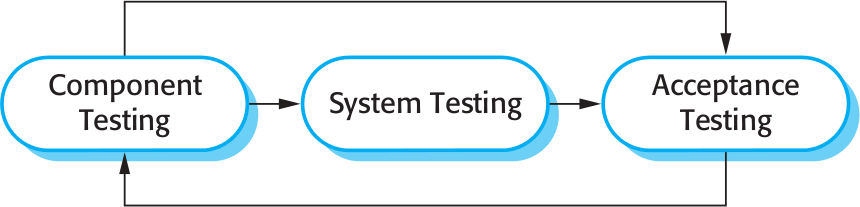
\includegraphics[width=0.75\textwidth]{mainmatter/pics/vandv.png}
  \caption{Testing Zyklus}
\end{figure}
\begin{itemize}
    \item Komponenten Testing:
    \begin{itemize}
        \item Tests von Einzelkomponenten unabhängig von einander
        \item Komponenten können Funktionen, Objekte oder kohärente Gruppen von Personen sein
    \end{itemize}
    \item Systemtest
    \begin{itemize}
        \item Test des gesamten Systems (entstehender Eigenschaften)
        \item Prüfung von emergenten Eigenschaften besonders wichtig
    \end{itemize}
    \item Abnahmetests:
    \begin{itemize}
        \item Testen mit Daten des Kunden zur Überprüfung der Anforderungen
    \end{itemize}
\end{itemize}
\begin{figure}[h]
  \centering
     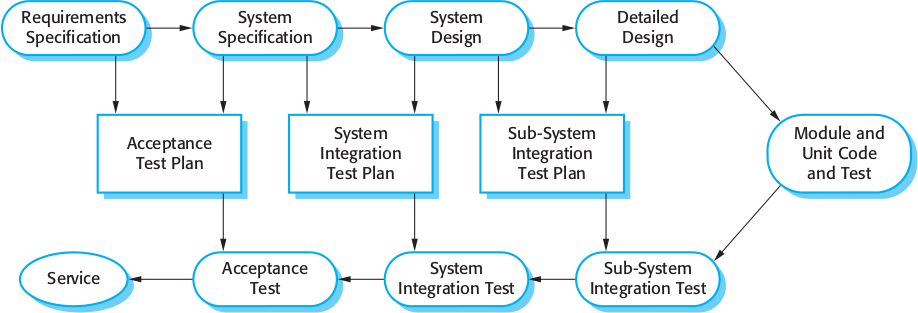
\includegraphics[width=0.75\textwidth]{mainmatter/pics/validation.png}
  \caption{Testing bei plangesteuertem Software-Prozess}
\end{figure}

\subsection{Software-Evolution}
\begin{itemize}
    \item Software ist von Natur aus flexibel und kann sich verändern
    \item Anforderungen änder sich durch wirtschafliche Umstände, die unterstützende Software muss sich mit verändern
    \item Durch die Wiederverwendung von Komponenten für neue Systeme sind Softwareentwicklung und Evolution nicht mehr vollständig unterscheidbar
\end{itemize}
\begin{figure}
    \centering
    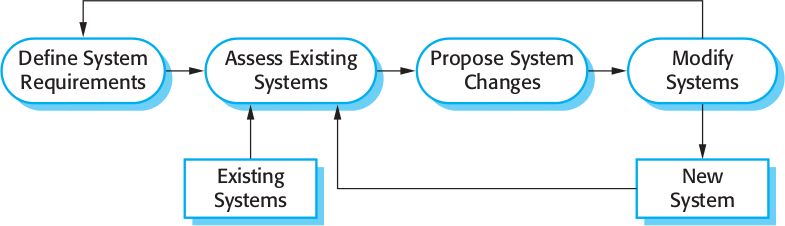
\includegraphics[width=0.75\textwidth]{mainmatter/pics/evolution.png}
    \caption{Software-Evolution}
\end{figure}

\subsection{Prototyping}
\begin{figure}
    \centering
    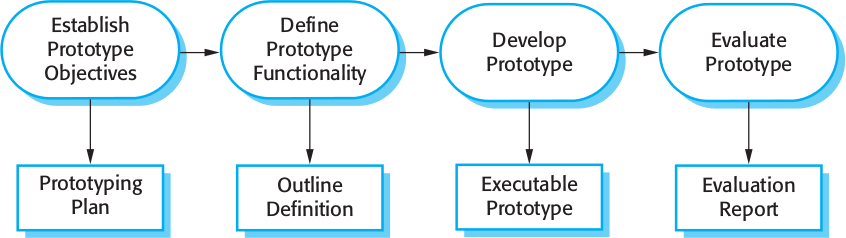
\includegraphics[width=0.75\textwidth]{mainmatter/pics/prototyping.png}
    \caption{Prototyping}
\end{figure}
\begin{itemize}
    \item eine erste Version eines Softwaresystems um Konzepte zu demonstrieren und Erkenntnisse zu gewinnen
    \item Wird benutzt, wenn:
    \begin{itemize}
        \item Requirements-Engineering Prozess hilft ein Prototyp bei der Ermittlung und Validierung der Systemanforderungen
        \item Beim Systementwurf kann der Prototyp verwendet werden, um einzelne Softwarelösungen zu utnersuchen und den Entwurf der Benutzeroberfläche zu unterstützen 
    \end{itemize}
\end{itemize}


\subsection{Spiralmodell nach Boehm:}
\begin{figure}
    \centering
    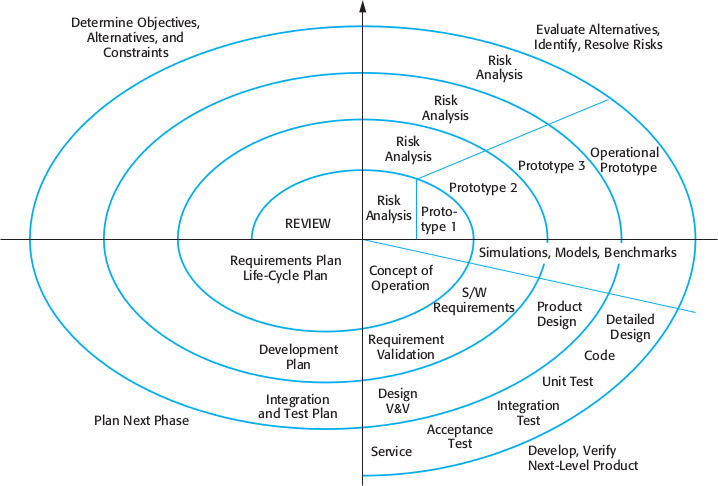
\includegraphics[width=12.5cm]{mainmatter/pics/boehm.png}
    \caption{Prototyping}
\end{figure}
\begin{itemize}
    \item Softwareprozess wird als Spirale dargestellt, anstatt als eine Folge von Aktivitäten 
    \item Jede Windung steht für eine Phase des Prozesses
    \item keine festen Phasen wie Spzeifikation $\rightarrow$ Schleifen werden nach Erforderlichkeit gewählt.
    \item beinhaltet explizite Risikomanagmentaktivitäten
    \item Jede Windung der Spirale ist in vier Segmente aufgeteilt:
    \begin{itemize}
        \item Ziele aufstellen
        \item Risiken einschätzen und verringern
        \item Entwicklungnd Validierung
        \item Planung
    \end{itemize}
    \item Nutzung:
    \begin{itemize}
        \item sehr einflussreich um Menschen zu helfen über Iterationen in Softwareprozessen und die Eifnührung des risikoorientierten Ansatzes für die Entwicklung nach zu denken
        \item Praxis
        \begin{arrowlist}
            \item Modell wird selten verwendet
            \item wird zur Veröffentlichung der praktischen Softwareentwicklung verwendet
        \end{arrowlist}
    \end{itemize} 
\end{itemize}

\subsection{Rational Unified Process (RUP):}
\begin{itemize}
    \item abgeleitet von der Arbeit an der UML
    \item Vereinigt Elemente aus allen allgemeinen \textbf{Vorgehensmodellen} (Wasserfall, inkrementelle Entwicklung und wiederverwendungsorienteirte SE)
    \item veranschaulicht empfohlene Vorgehensweisen für Spezifikation und Entwurf
    \item unterstützt Entwicklung von Prototypen
    \item RUP wird aus drei Perspektiven beschrieben
    \begin{itemize}
        \item \textbf{dynamische Perspektive:}\\
        die die Phasen des Modells zeitlich darstellt
        \item \textbf{statische Perspektive:}\\
        die die ausgeführten Prozessaktivitäten darstellt
        \item \textbf{praxisbezogene Perspektive:}\\ die die während des Prozesses empfohlene Vorgehensweise vorschlägt
    \end{itemize}
    \item Sechs grundlegende Vorgehensweisen für das SE zum Einsatz bei der Systementwicklung:
    \begin{enumerate}
        \item Software iterativ entwickeln:
        \begin{itemize}
            \item schrittweise Planung des Systems ausgehend von den Prioritäten des Kunden 
        \end{itemize}
        \item Anforderungen verwalten:
        \begin{itemize}
            \item Eindeutige Dokumentation der Kundenanforderungen
            \item geänderte Anforderungen verfolgen
        \end{itemize}
        \item Komponentenbasierte Architekturen verwenden:
        \begin{itemize}
            \item Aufteilung der Systemarchitektur in Komponenten (Wiederverwendung)
        \end{itemize}
        \item Software visuell modellieren:
        \begin{itemize}
            \item Verwenden grafischer UML-Modelle für dynamische und statische Sicht 
        \end{itemize}
        \item Softwarequalität verifizieren:
        \begin{itemize}
            \item Sicherstellen, dass die Software die Qulaitätsstandards des Unternehmens erfüllen
        \end{itemize}
        \item Änderungen der Software steuern (überprüfen):
        \begin{itemize}
            \item Verwaltung der Softwareveränderungen mithilfe eines Änderungsmanagementsystems
        \end{itemize}
    \end{enumerate}
\end{itemize}

		\chapter{Projekt Management}
\section{Einleitung}
\subsection{Erfolgskriterien}
\begin{enumerate}
    \item Ausliefern der Sfotware zur vereinbarten Zeit
    \item Budget einhalten
    \item Software erfüllt Anforderungen 
    \item gute Personalführung
\end{enumerate}
\begin{itemize}
    \item Besonderheiten:
    \begin{itemize}
        \item Software ist nicht greifbar, Fortschritt kann nicht direkt beobachtet werden
        \item Softwareprojekte unterscheiden sich stark voneinander $\rightarrow$ Probleme schwer abschätzbar
        \item \textbf{Softwareprozesse sind variabel un organisationssepzifisch}, Probleme sind immer noch schwer vorherzusagen
    \end{itemize}
\end{itemize}

\subsection{Management activities}
\begin{enumerate}
    \item \textbf{Angebot schreiben}
    \begin{itemize}
        \item Beschreibung der Projektziele, Vorgehenweise \dots $\rightarrow$ einholen von Aufträgen
    \end{itemize}
    \item \textbf{Projektplanung}
    \begin{itemize}
        \item Planung, Abschätzung des Aufwandes und Erstellung eines Zeitplanes
    \end{itemize}
    \item \textbf{Berichterstattung}
    \begin{itemize}
        \item Kunden und Management müsse über Fortschritt des Projektes unterrichtet werden
     \end{itemize}
     \item \textbf{Risikomanagement}
     \begin{itemize}
        \item abschätzen, beobachten und behandeln von Risiken
    \end{itemize}
    \item \textbf{Personalführung}
    \begin{itemize}
        \item Auswahl von Mitarbeitern und Herstellung von produktiven Arbeitspozessen
    \end{itemize}
\end{enumerate}

\section{Risikomanagement}
\begin{itemize}
    \item Identifikation von Risiken und entwickeln von Plänen zur Minimierung ihrer Effekte auf das Projekt 
    \item \textbf{Risiko: Warscheinlichkeit, dass negative Umstände eintreten}
    \item Risikobereiche
    \begin{itemize}
        \item \textbf{Projektrisiken} beeinflussen Zeitplan oder Mittel
        \item \textbf{Produktrisiken} beeinflussen Qualität oder Leistung der entwickelten Software 
        \item \textbf{Business risks} beeinflussen das Unternehmen, welches die Software entwickelt 
    \end{itemize}
    \item Vier Schritte:
    \begin{enumerate}
        \item \textbf{Risikoerkennung} \\
        (Projekt-, Produkt- und Unternehmensrisiken)
        \item \textbf{Risikoanalys}\\
        (Wahrscheinlihckeit und Folgen)
        \item \textbf{Risiko-Planung}\\
        (Vermeiden oder klein halten)
        \item \textbf{Risikobeobachtung}\\
        (Beobachtung während dem Projekt)
    \end{enumerate}
\end{itemize}

\subsection{Key Points:}
\begin{itemize}
    \item Gutes Projektmanagement ist entscheidend für die Einhaltung von Zeitplan und Budget
    \item Software ist nicht greifbar, Projekte können neuartig sein (keine Erfahrungswerte), Sfotwareentwicklung ist eine vergleichsweise neue Disziplin
    \item Risikomanagement beinhaltet Identifikation und Beurteilung von Projektrisiken ur Abschätzung der Wahrscheinlichkeit ihres Aufretens und ihrer möglichen Auswirkungen auf das Projekt 
    \item Vermeidung, Kontrolle oder umgang von wahrscheinlichen Risiken muss in die Planung miteinbezogen werden 
\end{itemize}

\section{Personalführung}
\subsection{Faktoren}
\begin{itemize}
    \item \textbf{Konsequenz:} Temamitglieder sollten alle gleich behandelt werden 
    \item \textbf{Respekt:} Unterschiedlihe Fähigkeiten der Teammitglieder sollten berückstichtigt werden 
    \item \textbf{Einbeziheung:} Alle Teammitglieder sollten in den Prozess miteinbezogen werden
    \item \textbf{Ehrlichkeit:} Ehrlichkeit bei Lob \& Kritik
\end{itemize}

\subsection{Motivation}
\begin{itemize}
    \item Organisation von Arbeit und ARbeitsumgebung, so dass Mitarbeiter zu effektiver ARbeit motiviert werden 
    \item Verschiedene formen von Motivation, je nach zugrundliegendem Bedürfnis
    \begin{itemize}
        \item Grundbedürfnisse (Essen, Schlafen, \dots)
        \item persönliche Bedürfnisse (Respekt, Selbstbewusstsein, \dots)
        \item soziale Bedürfnisse (akzeptiert werden, \dots)
    \end{itemize}
    \item Motivation sollte die verschiedenen Persönlichkeitstypen berücksichtigen
\end{itemize}

\subsection{Gruppenzusammensetzung}
\begin{itemize}
    \item Alle Persönlichkeitstypen sollten gleichermaßen vorhanen sein
    \begin{itemize}
        \item Aufgaben-orientiert: die Motivation für die Tätigkeit ist die Tätigkeit selbst
        \item Selbstbezogen: Arbeit ist Mittel zum Zweck
        \item Interaktions-orientiert: Hauptmotivation ist Anwesenheit und Mitarbeit von Kollegen
    \end{itemize}
    \item Interaktionsorientierte Persönlichkeiten besonders wichtig
\end{itemize}

\subsection{Key Points:} 
\begin{itemize}
    \item Menschen werden durch utnerschiedliche Dinge motiviert ( Interaktion, Anerkennung, Möglichkeiten zur persönlichen Weiterentwicklung)
    \item Gruppen sollten relativ klein und zusammenhängend sein, Gruppenzusammenhalt abhängig von Mitgliedern, Organisation und Kommunikation
    \item Gruppeninterne Kommunikation abhängig vom Status der Gruppenmitglieder, Gruppengröße, Geschlechterverteilung, Persönlichkeiten und Kommunikationswegen
\end{itemize}

\section{Projektplanung} 
\begin{itemize}
    \item Aufgabe einteilen und diese den Teammitgliedern zuweisen, Probleme vorhersehen und Lösungsmöglichkeiten vorbereiten
    \item Projektplan als Kommunikationsmittel mit Teammitgliedern und Kunden, bewerten des Fortschritts
    \item \textbf{Planungsstufen:}
    \begin{itemize}
        \item Angebotsstufe (nur Entwurf der Software Requirements $\rightarrow$ Preisgestaltung)
        \item Anfangsstufe des Projektes
        \item regelmäßig während des Projektes
    \end{itemize}
\end{itemize}

\subsection{Preisgestaltung: Faktoren}
\begin{itemize}
    \item Kostenabschätzung für den Entwickler
    \item organisatorische, wirtschaftliche, politische und unternehmensbezogene Erwägungen
\end{itemize}
\begin{enumerate}
    \item Marktchancen (niedrigerer Preis $\rightarrow$ Eroberung neuer Marktsegmente)
    \item Unsicherheit bei der Kostenabschätzung (Preis zur Sicherheit höher angesetzt)
    \item Vertragsbedingungen (niedrigerer Preis, wenn Rechte am Quelcode beim Entwickler bleiben)
    \item Unbeständigkeit der Anforderungen (zunächst niedriger Oreis, nach Fertigstellung hohe Gebhren für die Umsetzung von Änderungen)
    \item finanzielle Lage (besser geringer oder kein Gewinn als Insolvenz)
\end{enumerate}

\subsection{Plangesteuerte Entwicklung}
\begin{itemize}
    \item Alle Prozessaktivitäten von Anfang an geplant, Fortschritt an dieser Planung gemessen
    \item \textbf{Vorteile}
    \begin{itemize}
        \item verbesserte Organisation durch frühe Planung 
        \item mögliche Probleme und Abhängigkeiten fallen vor Projektbeginn auf 
    \end{itemize}
    \item \textbf{Nachteile}
    \begin{itemize}
        \item viele frühe Entscheidungen müssen später revidiert werden (veränderte Anforderunger/bedingungen)
    \end{itemize}
    \item \textbf{Projektplan}
    \begin{itemize}
        \item \textbf{Was} wird \textbf{von wem wann mit welchem Werkzeugen} getan? 
    \end{itemize}
\end{itemize}

\subsubsection{Abschnitte:}
\begin{enumerate}
    \item Einleitung 
    \item Projektorganisation
    \item Risikoanalyse
    \item Hardware- und Softwareanforderungen
    \item Arbeitseinteilung
    \item Zeitplan 
    \item Überwachungs- und Berichterstattungsmechanismen
\end{enumerate}

\subsubsection{Zeitplanung}
\begin{itemize}
    \item Abschätung der von jedem Arbeitsschritt benötigten Zeit und desbenötigten Arbeitsaufwandes.
    \item Abschätzung der benötigten Ressourcen (Hardware, finanziell)
\end{itemize}

\subsubsection{Arbeitsschritte:}
\begin{enumerate}
    \item Aufteilung des Projektes in Arbeitsschritte, Abschätzung der benötigten Zeit und Ressourcen
    \item Arbeitsschrite gleichzeitig ausführen lassen $\rightarrow$ optimale Ausnutzung der Arbeitskraft
    \item Minimierung von Abhängigkeiten zwischen den Arbeitsschritten $\rightarrow$ weniger Zeitverlust durch Wartezeiten
\end{enumerate}

\begin{figure}[h]
    \centering
    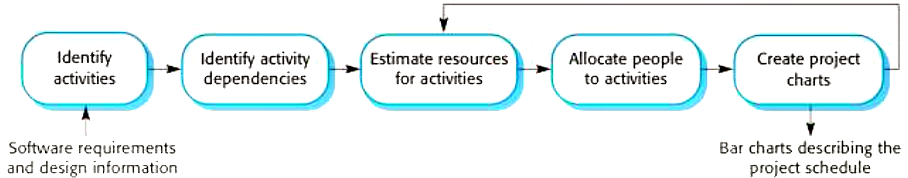
\includegraphics[width=0.75\textwidth]{mainmatter/pics/project_shedulding.png}
    \caption{Project schedulding}
\end{figure}

\subsubsection{Milestones und Deliverables:}
\begin{itemize}
    \item \textbf{Milestones:} Punkte im Zeitplan, dienen zur Bewertung des Fortschrittes
    \item \textbf{Deliverables:} Erzeugnisse, die an den Kunden ausgeliefert werden (Requirements documents)
\end{itemize}

\subsubsection{Probleme:}
\begin{itemize}
    \item Abschätzung des Ausmaßes von Problemen und damit der Kosten für ihre Lösung ist schwierig
    \item Produktivität ist nicht proportional zur Auswahl der Mitarbeiter 
    \item Einsatz von zusätzlichen Arbeitskräften bei einem verspäteten Projekt führt zu zusätzlicher Verspätung (Kommunkations-Overhead)
    \item Murphy's Law: möglichst alle Eventualitäten einplanen
\end{itemize}

\subsection{Agile Planung: Schritte}
\begin{itemize}
    \item \textbf{Agile Planung:} inkrementelle Planung, Prozess kann bei veränderten Anforderungen abgeändert werden
    \item \textbf{Planung der Veröffentlichung:} mehrere Monate im Voraus, bestimmt die in der Veröffentlichung inbegriffenen Funktionen
    \item \textbf{Planung der Iterationen:} kurzfristig, Planung es nächsten Inkrements (2-4 Wochen Arbeitszeit)
    \item \textbf{Extreme Programming (XP):} Story-basierte Planung 
\end{itemize}

\subsection{Key Points:}
\begin{itemize}
    \item Preis für Software wird nicht nur durch Entwicklungskosten bestimmt, sondern kann durch Markt- oder Unternehmensprioritäten beeinflusst werden. 
    \item Planungsgesteuertes entwickeln wird um inen kompletten Projektplan organisiert, definiert Projektaktivitäten, Aufwand, Zeitplan und Aufgabenverteilung
    \item Erstellung des Zeitplans mit Hilfe von graphischen Darstellungen des Projektplans 
    \item XP-Planspiel beteiligt das gesamte Team an der Projektplanung. Plan wird inkrementell entwickelt, wird bei auftretenden Problemen angepasst (Reduzierung von Funktionalitäten anstatt Verzögerung der Auslieferung)
\end{itemize}

\section{Techniken zur Aufwandsabschätzung}
\textbf{\large{Zwei Arten:}}
\begin{itemize}
    \item \textit{Erfahrungsbasiert:} Abschätzung des benötigten Aufwandes abhängig von Erfahrung des Projektleiters und des Anwendungsbereiches der Software 
    \item \textit{Algorithmische Kostenmodellierung:} formelähnliche Herangehensweise zur berechnung des Arbeitsaufwandes, basierend auf Abschätzung von Projektattributen (Größe, Erfahrung der Mitarbeiter, \dots)
\end{itemize}

\subsection{Algorithmische Kostenmodellierung}
\begin{itemize}
    \item Mathematische Funktion aus Produkt, Projekt, Prozessatributen. Werte werden vom Projektleiter abgeschätzt
    \item $A \times Size^{B} \times M$
    \begin{itemize}
        \item $A$: organisationsabhägige Konstante
        \item $B$: spiegelt den uvnerhätlnismäßigen Aufwand für große Projekte wieder
        \item $M$: Multiplikator, spiegelt Produkt-, Pozess- und Personalattribute wieder 
    \end{itemize}
    \item \textcolor{red}{Häufigstes Produktattribut: Codegröße}
    \item Modelle meist ähnlich, aber unterschiedliche Werte für $A$, $B$ und $M$
\end{itemize}

\subsection{Genauigkeit der Abschätzung}
\begin{itemize}
    \item Größe einer Sfotware erst nach Fertigstellung bekannt
    \item beeinflussende Faktoren:
    \begin{itemize} 
        \item Verwendung von COTS und bereits existierenden Komponenten 
        \item Programmiersprache
        \item Verteilung des Systems
    \end{itemize}
    \item je weiter der Entwicklungsprozess fortgeschritten ist, desot genauer kann die codegröße abgeschätzt werden 
    \item Abschätzungen der zu $B$ und $M$ gehörenden Faktoren subjektiv
\end{itemize}

\subsubsection{COCOMO 2}
\begin{itemize}
    \item empirisches Modell, erfahrungsbasiert
    \item gut dokumentiert, unabhängig
    \item mehrfah überarbeitet
    \item berückstichtigt verschiedene Herangehensweisen an softwareentwicklung, Wiederverwendung etc.
    \item enthält eine Anzahl von Untermodellen $\rightarrow$ zunehmend detailliertere Abschätzungen 
    \item Untermodelle:
    \begin{enumerate}
        \item \textbf{Application-composition-Modell} \\
        zusammensetzen von Software aus bereits existierenden Teilen
        \item \textbf{Frühes Designmodell} \\
        Anforderungen verfügbar, aber Designprozess noch nicht begonnen
        \item \textbf{Reuse-Modell} \\
        Berechnung des Aufwandes, wiederverwendbare Komponenten zu integrieren
        \item \textbf{Post-architecture-Modell}\\
        nach Design der Systemarchitektur $\rightarrow$ mehr Infromation über das System verfügbar
    \end{enumerate}
\end{itemize}
\begin{figure}[h]
    \centering
    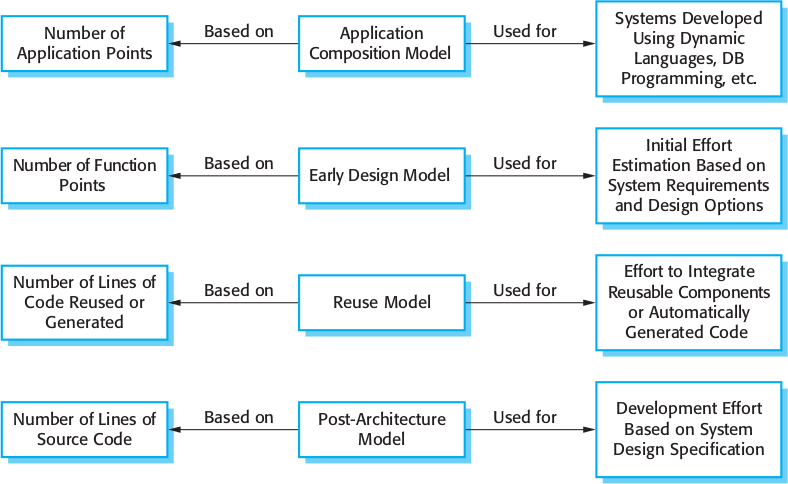
\includegraphics[width=0.75\textwidth]{mainmatter/pics/cocomo.png}
    \caption{COCOMO estimation models}
\end{figure}

\subsubsection{Application composition-Modell}
\begin{itemize}
    \item Prototypenentwicklung, Projekte mit viel Wiederverwendung 
    \item \textbf{standard estimates of developer productivity in application (oject) points/month}
    \item Nutzung von CASE berücksichtigen
    \item \textbf{Gleichung:} $PM = (NAP \times (1-\%reuse/100))/PROD$
    \begin{itemize}
        \item $PM$: Aufwand (Monate Arbeitszeit pro Person) 
        \item $NAP$: Anzahl der application points 
        \item $PROD$: Produktivität
    \end{itemize}
\end{itemize}

\subsubsection{Frühes Designmodell}
\begin{itemize}
    \item Abschätzung nach Einigung über Anforderungen 
    \item basiert auf Standartformel für algorithmische Modelle: 
    \begin{itemize}
        \item $PM = A \times Size^{B} \times M$
        \begin{itemize}
            \item $M = PERS \times RCPX \times RUSE \times PDIF \times PREX \times FCIL \times SCED$
            \item $A$: beginnt bei 2.94 [KLOC]
            \item $B$: 1.1 - 1.24 (abhängig von Neuartigkeit des Projektes, Flexibilität der Entwicklung Risikomanagement, Reife des Prozesses)
        \end{itemize}
    \end{itemize}
\end{itemize}

\subsubsection{Multplikatoren}
\begin{itemize}
    \item Produktattribute
    \begin{itemize}
        \item geforderte Eigenschaften der Software 
    \end{itemize}
    \item Computer-Attribute
    \begin{itemize}
        \item Eisnchränkungen durch Hardware
    \end{itemize}
    \item Personalattribute
    \begin{itemize}
        \item Erfahrung und Fähigkeit der Entwickler
    \end{itemize}
    \item Projektattribute 
    \begin{itemize}
        \item Eigenschaften des Entwicklungsprozesses
    \end{itemize}
\end{itemize}

\subsection{Key Points:}
\begin{enumerate}
    \item Abschätzungs-Techniken für Software sind erfahrungsbasiert (Projektleiter bewerten den benötigten Aufwand) oder algorithmisch (Aufwand berechnet aus anderen abgeschätzten Projektparamtern)
    \item COCOMO 2 - Kostenberechnungsmodell: algorithmisches Modell, das Projekt-, Produkt-, Hardware- und Personalattribute, sowie Produktgröße und -komplexität beachtet
\end{enumerate}

		
	\backmatter
		\listoffigures 
\end {document}
